
\section{Zoeken}\label{zoeken}

\subsection{Suggesties}
\pvelist{ \pve{4.11.1} }
De bezoeker van de website ziet op elke pagina een zoekbox (rechtsboven). Wanneer men hier begint met typen verschijnen er suggesties. Deze suggesties worden automatisch aangemaakt a.d.v. trefwoorden die eerder zijn gebruikt. Deze trefwoorden worden pas als suggestie gebruikt wanneer deze minimaal 3 keer zijn gebruikt. Dat om te voorkomen dat spelfouten en andere ongewenste suggesties direct zichtbaar worden voor alle gebruikers.

Later kunnen ongewenste suggesties alsnog worden verwijderd. Tevens is het mogelijk om handmatig suggesties toe te voegen. Ga naar \emph{Inhoud} en klik op het tabblad \emph{Suggesties} of ga direct naar \drupalpath{admin/content/suggestions} om de lijst van suggesties in te zien. Klik naast een suggestie op \emph{verwijderen} om deze te verwijderen, of klik bovenaan de pagina op \emph{Nieuwe suggestie toevoegen} om een nieuwe suggestie aan te maken.

Wijzigingen worden elke nacht verwerkt en zijn dus niet direct zichtbaar voor de gebruiker.

\subsection{Uitsluiten contenttypes van indexatie}
Niet alle content moet in de zoekresultaten tevoorschijn komen. Via \drupalpath{/admin/config/search/apachesolr/settings/solr/index} kun je bepaalde contenttypes uitsluiten van indexatie. 

\begin{figure}[p]
\centering
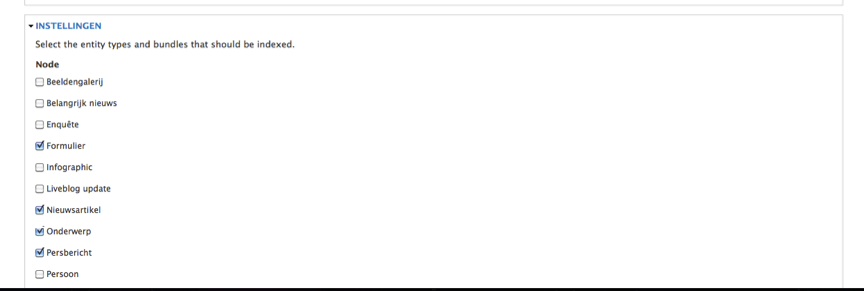
\includegraphics[width=\textwidth]{img/solr1.png}
\end{figure}

\subsection{Gebruik bias om zoekresultaten te beinvloeden}
Via de bias instellingen in de Apache Solr Search module kun je geindexeerde nodes een �score� geven in het zoekresultatenoverzicht. Deze bias instellingen kun je aanpassen via \drupalpath{/admin/config/search/apachesolr/settings}.

\begin{figure}[p]
\centering
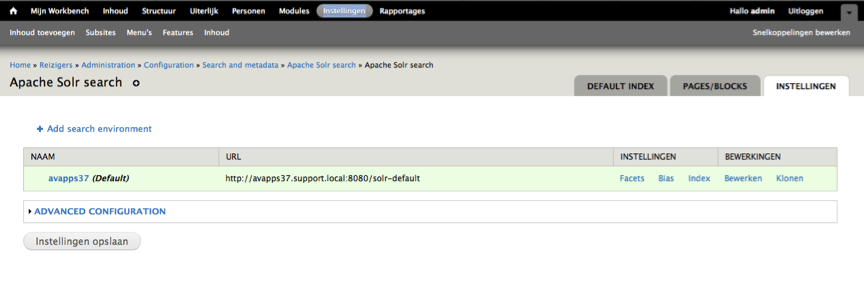
\includegraphics[width=\textwidth]{img/solr2.png}
\end{figure}

Zoek bias beinvloedt de importantie van bepaalde aspecten in de zoekresultaten.  Elke waarde behalve �Weglaten� of �Negeren� verhoogt de score van het betreffende aspect in de zoekresultaten. Hoe hoger de score, hoe groter de invloed op de zoekresultaten. De score die je als bias kan instellen varieert van 0.1 tot 21.0. Er zijn verschillende soorten bias instellingen:

\begin{itemize}
\item node attributes
\item content type
\item node fields
\end{itemize}

\subsection{Bias door node attributes}

\begin{figure}[p]
\centering
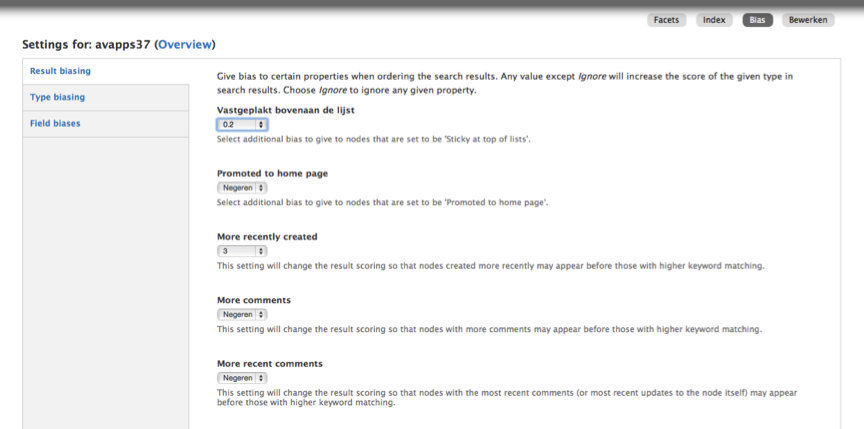
\includegraphics[width=\textwidth]{img/solr3.png}
\end{figure}

Via het tabblad Result biasing kun je bias toevoegen om nodes een hogere score te geven die  you can add search bias to favor nodes that are or have:

\begin{itemize}
\item Vastgeplakt zijn / Sticky gemaakt zijn
\item Naar de frontpage zijn gepromoveerd
\item Recenter zijn gepubliceerd
\item Meer reacties hebben
\item Meer recentere reacties hebben
\end{itemize}

\subsection{Bias door content type}
Via het tabblad Type biasing and exclusion kun je verschil in bias aangeven tussen bepaalde contenttypes ection. Zo kun je nieuwsberichten een hogere score geven dan bijvoorbeeld een statische pagina. 

\subsection{Bias door node fields}
Via het tabblad Field biases kun je de biasinstellingen aanpassen van verschillende velden van een node. Je kan bijvoorbeeld een hogere score geven als de zoekterm voorkomt in de H1 (oftewel titel) van een node. Dit kun je ook instellen voor een H2, H3, H4, bodytekst, reacties etc. 

Als je de score van een veld op �Weglaten� zet dan zal dit element niet meegenomen worden bij het bepalen van de volgorde van de zoekresultaten.

\begin{figure}[p]
\centering
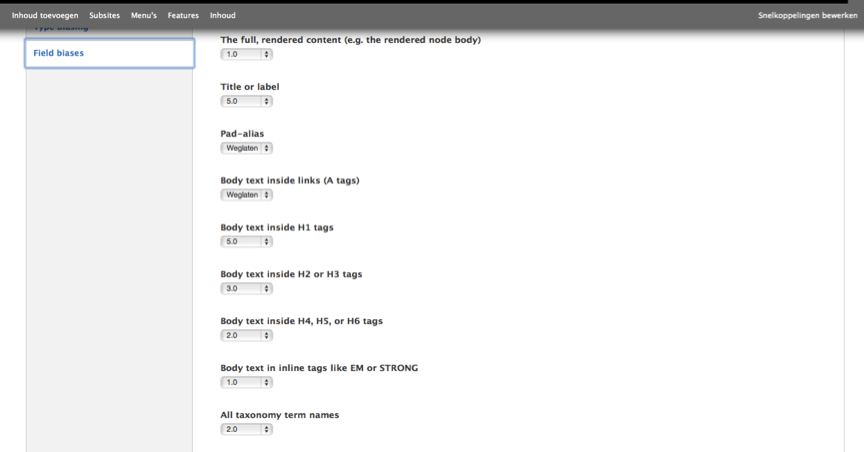
\includegraphics[width=\textwidth]{img/solr4.png}
\end{figure}



